%%%%%%%%%%%%%%%%%%%%%%%%%%%%%%%%%%
% Explanation of control regions
%%%%%%%%%%%%%%%%%%%%%%%%%%%%%%%%%%

The control regions are defined such that they are enriched in of the three main backgrounds in the
signal region, $t\bar{t}$, QCD multijet, and $\W(\rightarrow \ell \nu)+$jets. The control region
selections will be as close as possible to the signal selection, while maximizing the purity in a
given background process and minimizing possible signal contamination. 
To construct the control regions, different requirements on the 
multiplicity of leptons, $\cPqb$ tagged, and $\W$ tagged jets are placed. 
In the following subsections each control region will be discussed in detail. 

\subsubsection{\texorpdfstring{$T$}{T} region \label{sec:boost_T_region}}

The dominant background in the signal region is $t\bar{t}$ production. We define the $T$ region as a
dedicated control region enriched in this process. 
Similarly to the signal, $t\bar{t}$ events are expected to have $\cPqb$ jets in the final state, as
well as real hadronically decaying $\W$ bosons. We will thus not change those aspects of the signal
selection when defining the $T$ region. 

The main change we do make, is requiring the presence of exactly one loose electron or muon, while
removing the requirement that there be an isolated track. This selection is already sufficient to
obtain a region with a good purity of $t\bar{t}$ events. There is, however, a possibility of
substantial signal contamination. To address this issue, we place an upper boundary on the value of
the transverse mass, $\mT$, computed from the lepton transverse momentum and \VEtmiss, 
\begin{equation}
 \mT = \sqrt{2\pt^\ell\ETm ( 1 - \cos\Delta\phi )},
\end{equation}
with $\Delta\phi$ the difference in azimuthal angle between lepton and \VEtmiss. 
The distribution of $\mT$ exhibits a kinematic edge at the mass of the $\W$ boson for the $t\bar{t}$
process, an edge not present for signal events due to the extra contribution to the \ETm from the
invisible neutralinos.  We require $\mT < 100$\GeV in order to reduce signal contamination and
retain most of the $t\bar{t}$ contribution. The $\mT$ distribution at this selection level is shown
in Fig.~\ref{fig:boost_T_region_mT}. 

The final ingredient for the full $T$ region selection, is the $\Delta\phi_{min} > 0.5$
requirement. This is used to obtain a selection, and thus kinematic properties, as close as
possible to the signal region. A summary of the $T$ region selection is presented in
Table~\ref{tab:boost_selection_summary}. 

Table~\ref{tab:cutflow} shows a breakdown of the contributions of the various background components,
as determined directly from simulation, as wel as the observed data counts, and expected counts for
an example signal point. From Table~\ref{tab:BG_comp_percent} we see that the obtained purity in the
$T$ region is more than 80\% for $t\bar{t}$ and single top processes combined. This is also
illustrated in the $\mr$ and $\rsq$ distributions, as shown on Fig.~\ref{fig:boost_T_region_MR_Rsq}.
There is good agreement between data and simulation in the $T$ region. 
We also compare the shape of the $\mr$ and $\rsq$ distributions in the $T$ region versus the $S$
region. We observe from Fig.~\ref{fig:boost_T_region_shape} that the shapes are very similar. This
is important as we will use global transfer factors $\kappa$ to translate between the $T$ and $S$
regions. 


% Overall, there is a reasonable agreement between data and MC yields.  The mild discrepancies can
% be
% accommodated by the systematic uncertainties on the MC, and they will not affect our analysis.
% The control regions have a good purity for the background
% process they target: 90\% for multijet, 85\% for $\PW(\rightarrow \ell\nu)+$jets and close to 80\%
% for $t\bar{t}$ and single top processes combined. 


\begin{figure}[htbp]
\centering
% 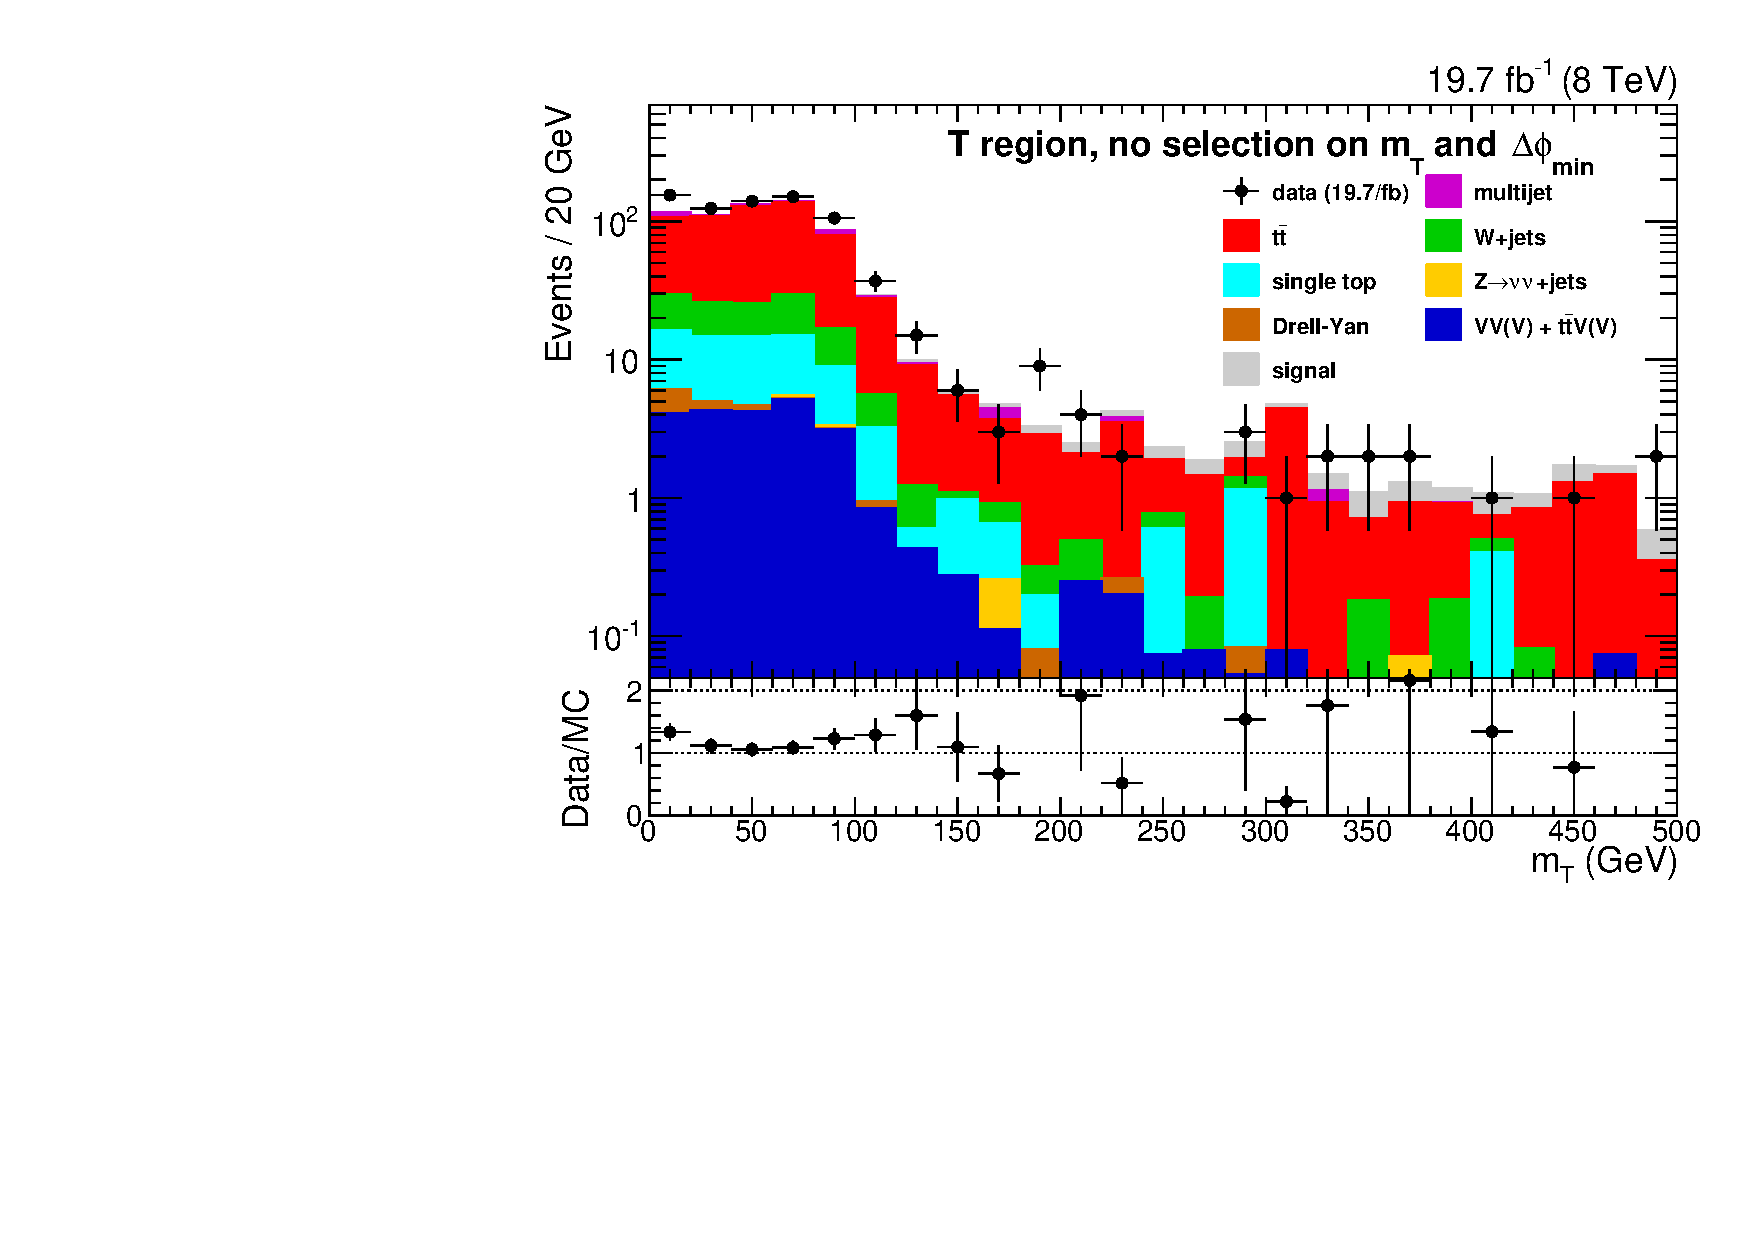
\includegraphics[width=0.7\textwidth]{figures/DataMC/DataMC_mT_g1Mbg1W1Ll_rebin}
\caption{Comparison between data and simulation of the $\mT$ distribution in the $T$ region without
any selection on $\mT$ or $\Delta\phi_{min}$. The kinematic edge at the $\W$ boson mass is clearly
visible for the SM backgrounds, whereas the example signal point extends out to high $\mT$.
\label{fig:boost_T_region_mT}}
\end{figure}

\begin{figure}[htbp]
\centering
% 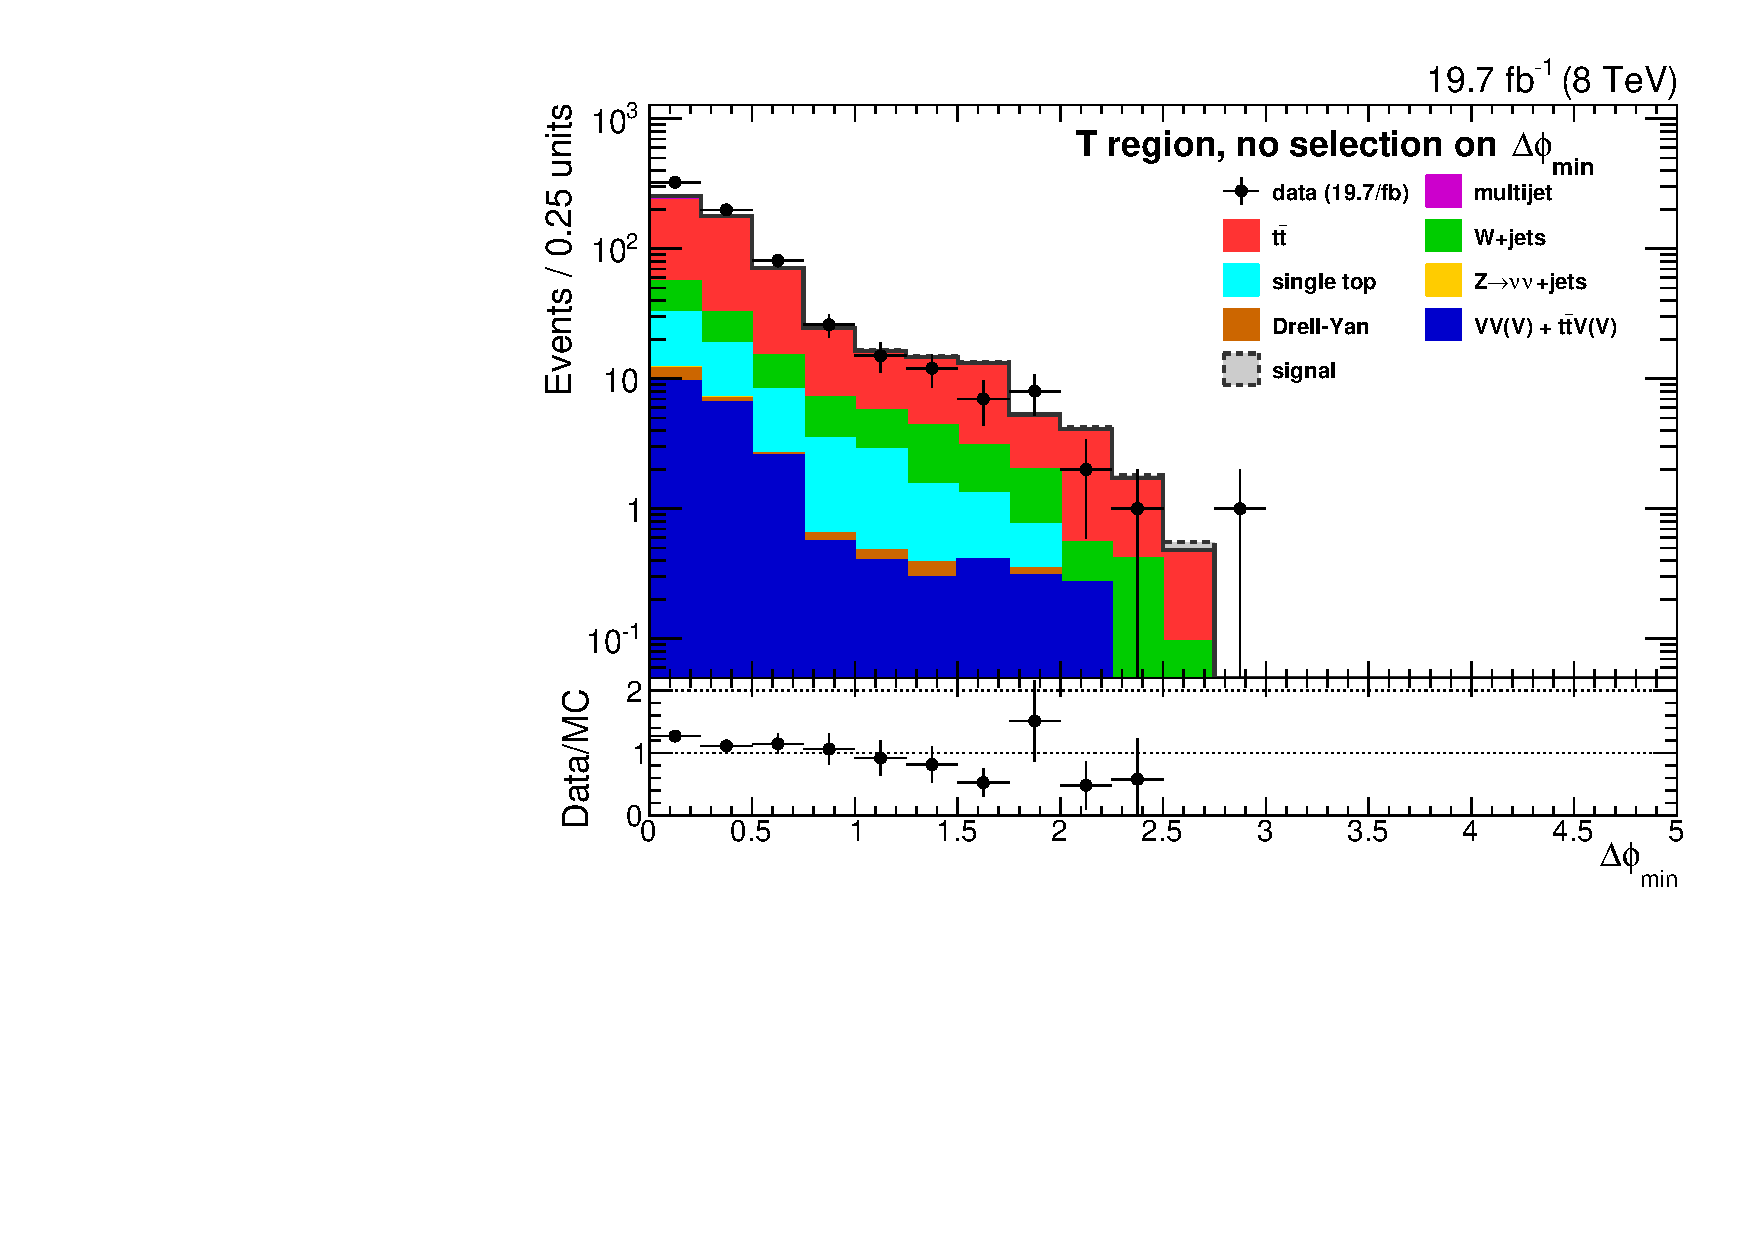
\includegraphics[width=0.49\textwidth]{figures/DataMC/DataMC_minDeltaPhi_g1Mbg1W1LlmT100_rebin}
\caption{Comparison between data and simulation of the $\Delta\phi_{min}$ distribution in the $T$
region without any selection on $\Delta\phi_{min}$.
\label{fig:boost_T_region_mindeltaphi}}
\end{figure}


% Comparisons between data and simulation  for various other basic quantities in
% figure~\ref{fig:DataMC_TRegion_mdphig0p5}. In figure~\ref{fig:Shape_TTJ_TvsS}, we show a comparison
% between the $M_R$ and $R^2$ shapes for TTjets simulation in the signal region versus the TTjets
% control region. The observed shapes are very similar. 
% 
\begin{figure}[htbp]
\centering
%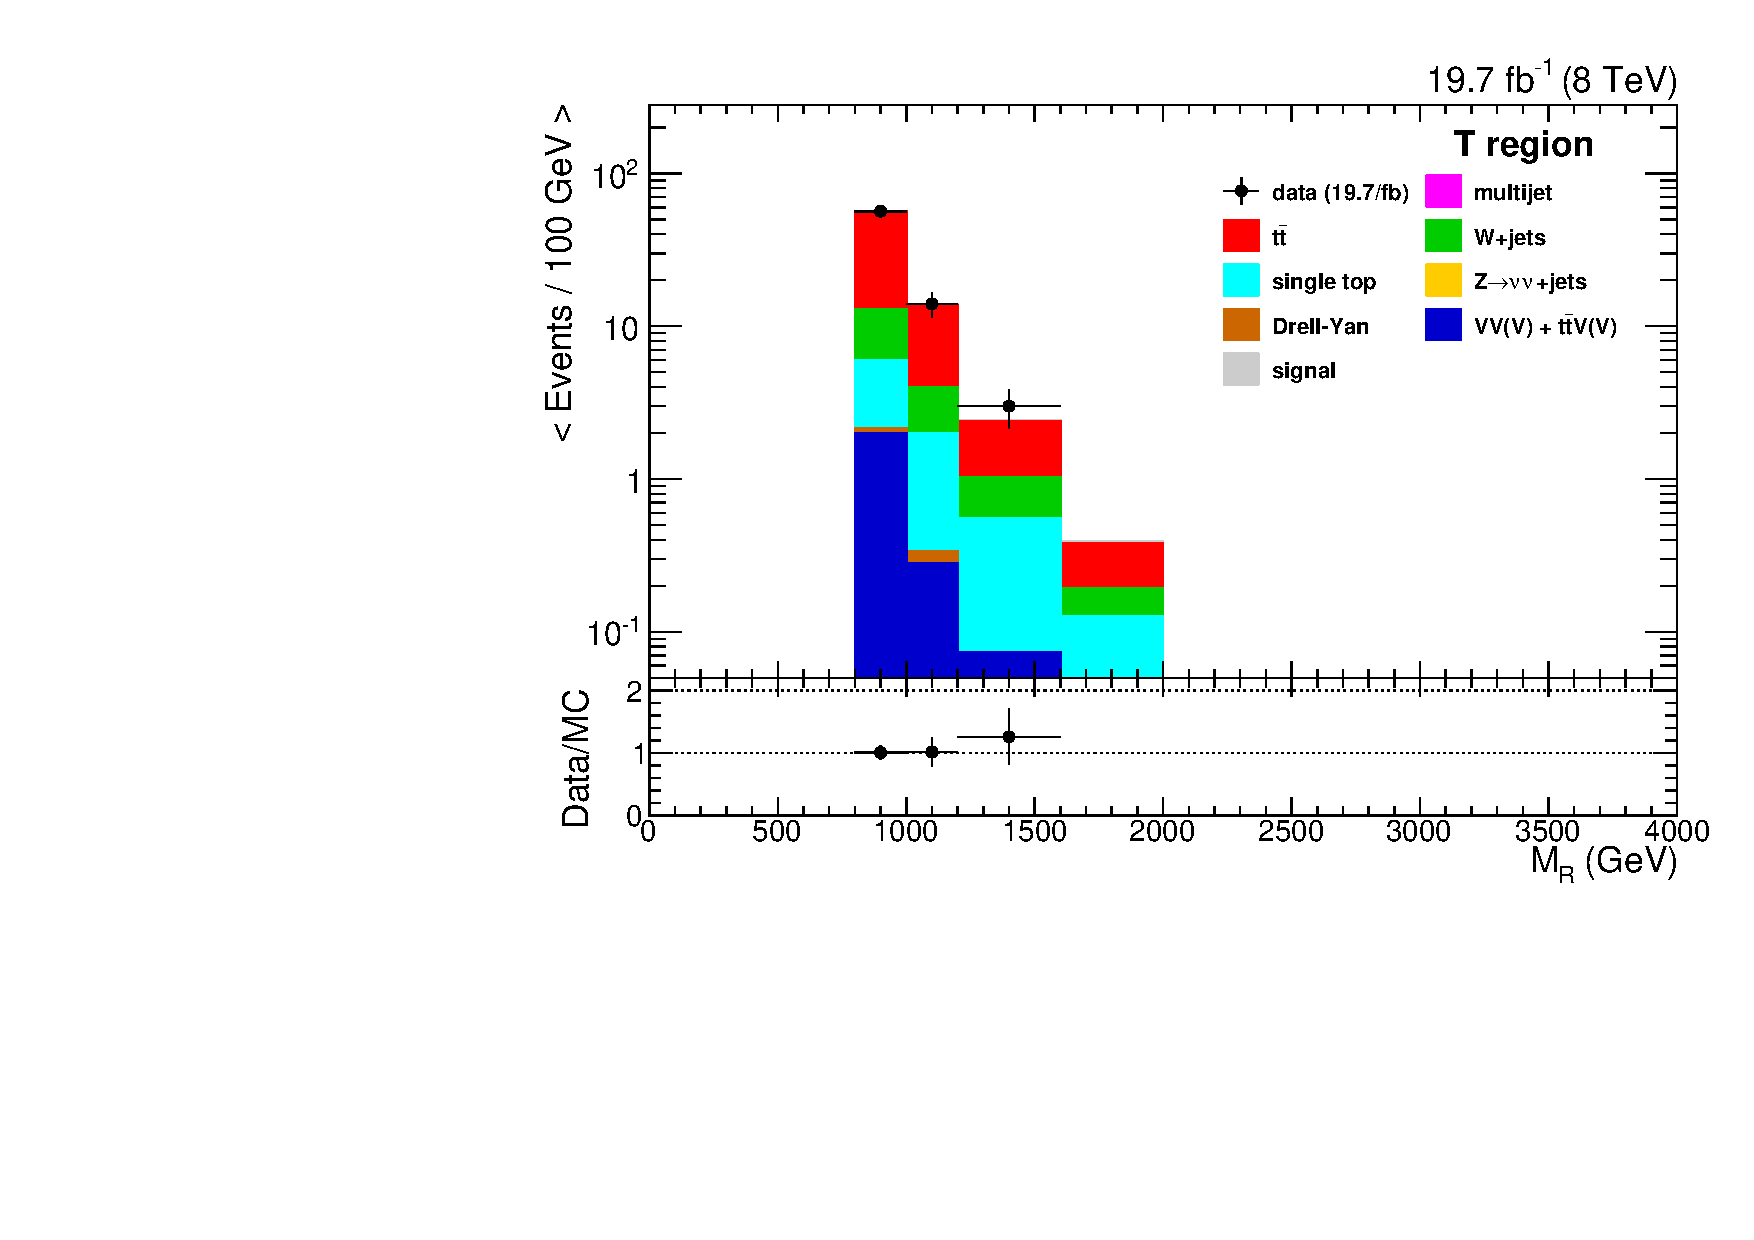
\includegraphics[width=0.48\textwidth]{figures/DataMC/DataMC_MR_g1Mbg1W1LlmT100_mdPhig0p5_width}
%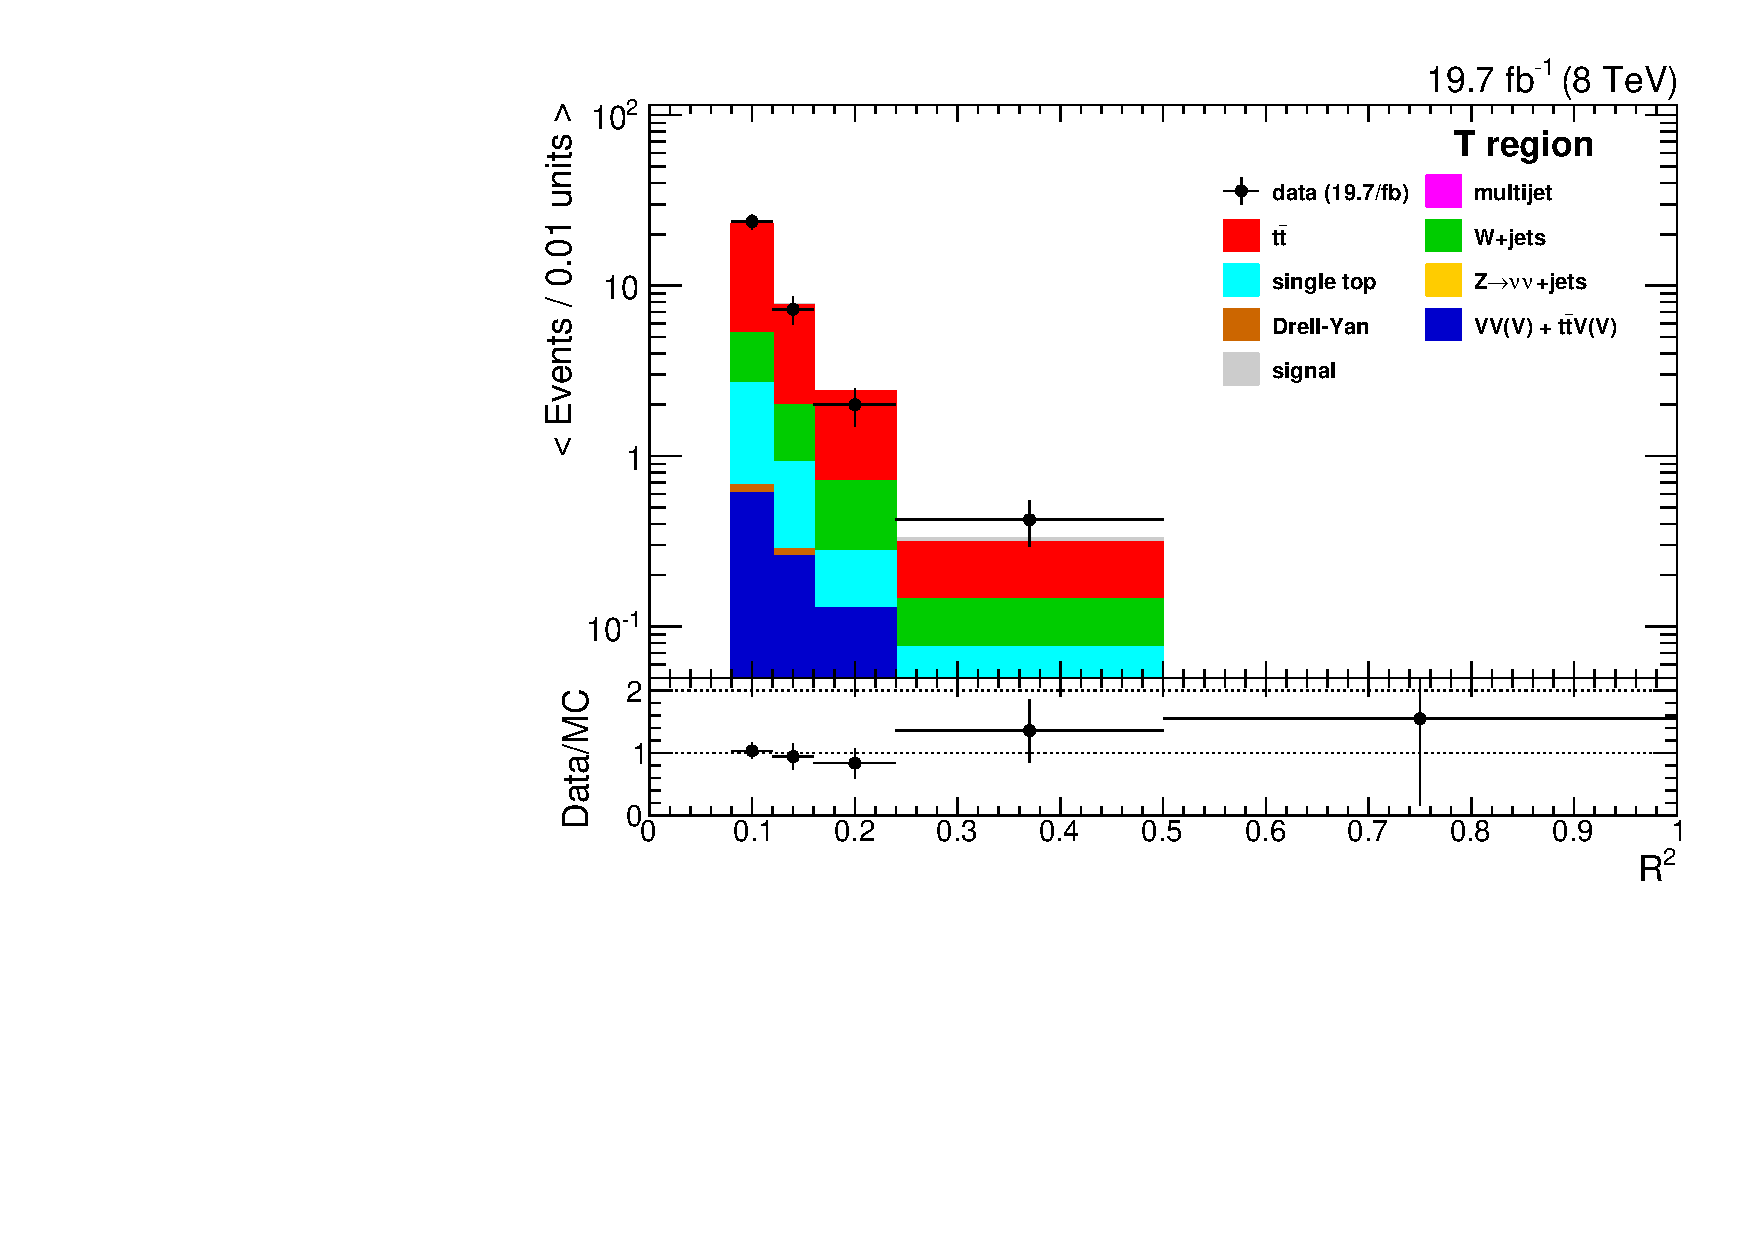
\includegraphics[width=0.48\textwidth]{figures/DataMC/DataMC_R2_g1Mbg1W1LlmT100_mdPhig0p5_width}
\caption{Comparison between data and simulation of the $\mr$ (left) and $\rsq$ (right)
distribution in the $T$ control region.
\label{fig:boost_T_region_MR_Rsq}}
\end{figure}
% 
% 
% \begin{figure}[p]
% \centering
%  \includegraphics[width=0.49\textwidth]{figures/DataMC/DataMC_njets_g1Mbg1W1LlmT100_mdPhig0p5}
%  \includegraphics[width=0.49\textwidth]{figures/DataMC/DataMC_nbjets_g1Mbg1W1LlmT100_mdPhig0p5}
% 
%  \includegraphics[width=0.49\textwidth]{figures/DataMC/DataMC_met_g1Mbg1W1LlmT100_mdPhig0p5}
%  \includegraphics[width=0.49\textwidth]{figures/DataMC/DataMC_jet1pt_g1Mbg1W1LlmT100_mdPhig0p5}
% 
%  \includegraphics[width=0.49\textwidth]{figures/DataMC/DataMC_jet2pt_g1Mbg1W1LlmT100_mdPhig0p5}
%  \includegraphics[width=0.49\textwidth]{figures/DataMC/DataMC_jet3pt_g1Mbg1W1LlmT100_mdPhig0p5}
% \caption{Data/MC comparison plot of various event quantities in the T region: 
% [top] jet multiplicity (left) and b-tagged jet multiplicity (right);
% [middle] missing transverse energy (left) and \pt of the highest \pt jet (right);
% [bottom] \pt of the second (left) and third (right) highest \pt jet. 
% \label{fig:DataMC_TRegion_mdphig0p5}}
% \end{figure}
% 

\begin{figure}[htbp]
\centering
%\includegraphics[width=0.48\textwidth]{figures/Shapes/MR_comparison_TTJ_TvsS_mdphi}
%\includegraphics[width=0.48\textwidth]{figures/Shapes/R2_comparison_TTJ_TvsS_mdphi}
\caption{Comparison of the shape of the $\mr$ (left) and $\rsq$ (right) distribution for the
$t\bar{t}$ simulation in the $T$ region versus the $S$ region. The histograms are normalized to
unit area. 
\label{fig:boost_T_region_shape}}
\end{figure}



%%%%%%%%%%%%%%%%%%%%%%%%%%%%%%%%%%%%%%%%%%%%%%%%%%%%%%%%%%%%%%%%%%%%%%%%%%%%%%%%%%%%%%%%%%%%%%%%


\subsubsection{\texorpdfstring{$W$}{W} region}

The second largest background in the signal region comes from $\W(\rightarrow l\nu)$+jets
production, where the lepton from the $\W$ boson decay is lost.
Because the $\W$ boson decays leptonically, any events passing the signal selection necessarily
contain a q/g initiated CA8 jet that is misidentified as a boosted $\W$ boson. 
We do not expect hadronically decaying $\W$ bosons to contribute to the background in the signal
region, as those events would have very small missing energy, in addition to not having real
$\cPqb$ jets. Even though we do not explicitely require a minimal \ETm, our $\rsq$ cut is highly
correlated with \ETm, and induces a minimal cut of around 100\GeV, as can be seen in
figure~\ref{fig:DataMC_SignalRegion_mdphig0p5}.  
This expectation was verified by checking the contribution of $\W(\rightarrow
q\bar{q}')+b\bar{b}$ using simulation, where it was found that no events pass our signal
selection. 

In order to accurately model the $\W(\rightarrow l\nu)$+jets background, we define a dedicated
control region, the $W$ region, as similar to the signal region as possible. As for the $T$ region,
we require the presence of a loose electron or muon. Additionally we also veto any event that
contains a CSV loose $\cPqb$ tagged jet.  
Since for the $\W(\rightarrow l\nu)$+jets process, there is no real hadronically decaying $\W$
boson, we opt not to use the full $\W$ tagger. 
In order to increase the number of events available in the control region, we require instead the
presence of at least one $\W$ boson mass-tagged jet. This ensures that we are in a kinematically
similar phase space, because we keep the jet mass requirement, but prevents the penalty from
requiring a two-prong decay for a process for which these decays do not occur. 

We also require $\mT < 100$\GeV in order to reduce possible signal contamination. Unlike for the $T$
region, we additionally require $\mT > 30$\GeV in order to reduce remaining contamination from
multijet events. Those events generally have low $\ETm$, which translates in low $\mT$. 
Multijet contamination in the $T$ region is negligible because of the
requirement that there be at least one jet tagged a coming from a $\cPqb$ quark. 
Finally, we also require $\Delta\phi_{min} > 0.5$, as was the case for the signal region. 

Figure~\ref{fig:boost_W_region_mT} shows the $m_T$ distribution in the $W$ region before making any
selection $\mT$ or on $\Delta\phi_{min}$. The $\Delta\phi_{min}$ distribution in the $W$ region
without applying a selection on $\Delta\phi_{min}$ is given in
Fig.~\ref{fig:boost_W_region_mindeltaphi}. The full breakdown of the backgrounds in this region is
listed in Tables~\ref{tab:cutflow} and \ref{tab:BG_comp_percent}. The $W$ region is about 85\% pure
in the $\W(\rightarrow l\nu)+$jets process. 
A comparison between data and simulation for the $\mr$ and $\rsq$ distributions is shown in
Fig.~\ref{fig:boost_W_region_MR_Rsq}. A reasonable agreement is observed. The offset in the
normalization will be absorbed automatically during the background estimation procedure. 

\begin{figure}[htbp]
\centering
% 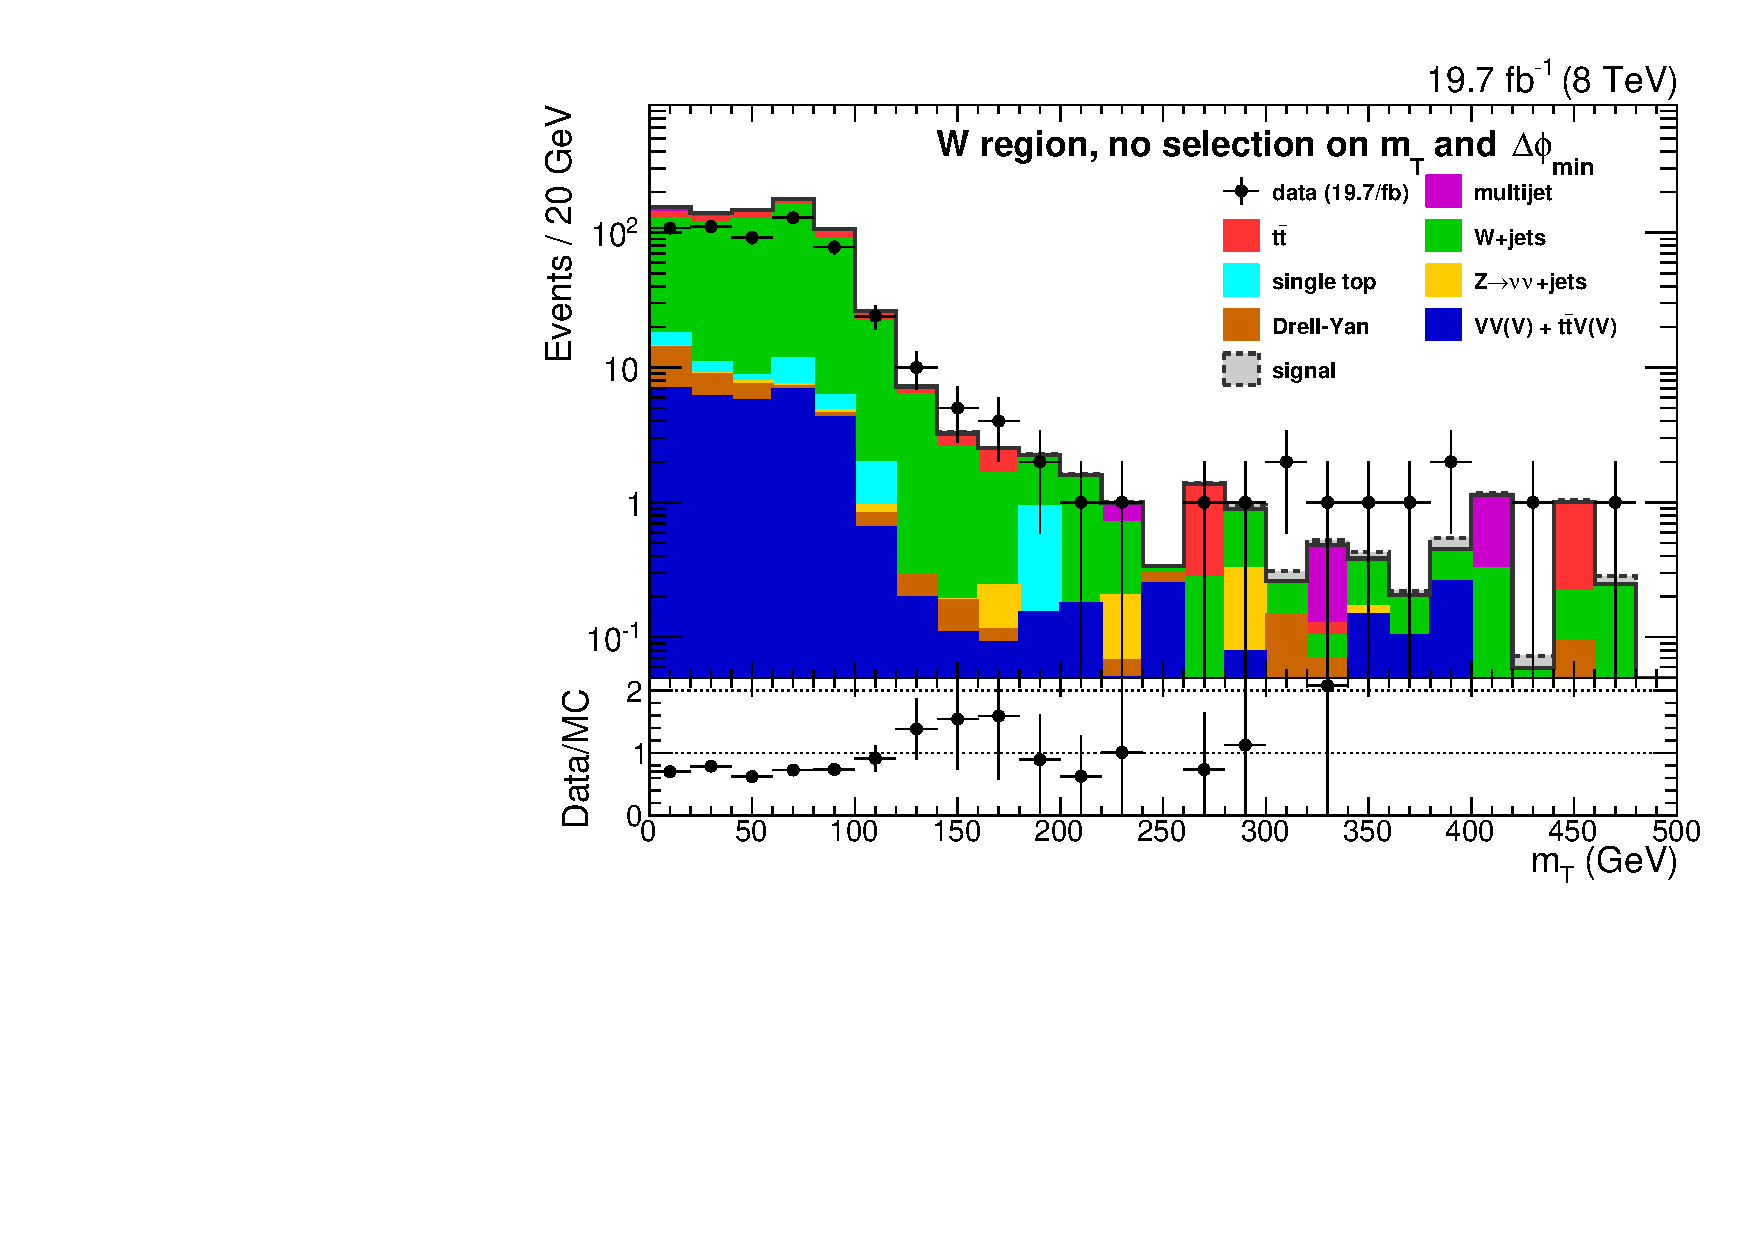
\includegraphics[width=0.6\textwidth]{figures/DataMC/DataMC_mT_0Lbg1Y1Ll_rebin}
\caption{Comparison between data and simulation of the $\mT$ distribution in the $W$ region without
any selection on $\mT$ or on $\Delta\phi_{min}$.
\label{fig:boost_W_region_mT}}
\end{figure}

\begin{figure}[htbp]
\centering
% 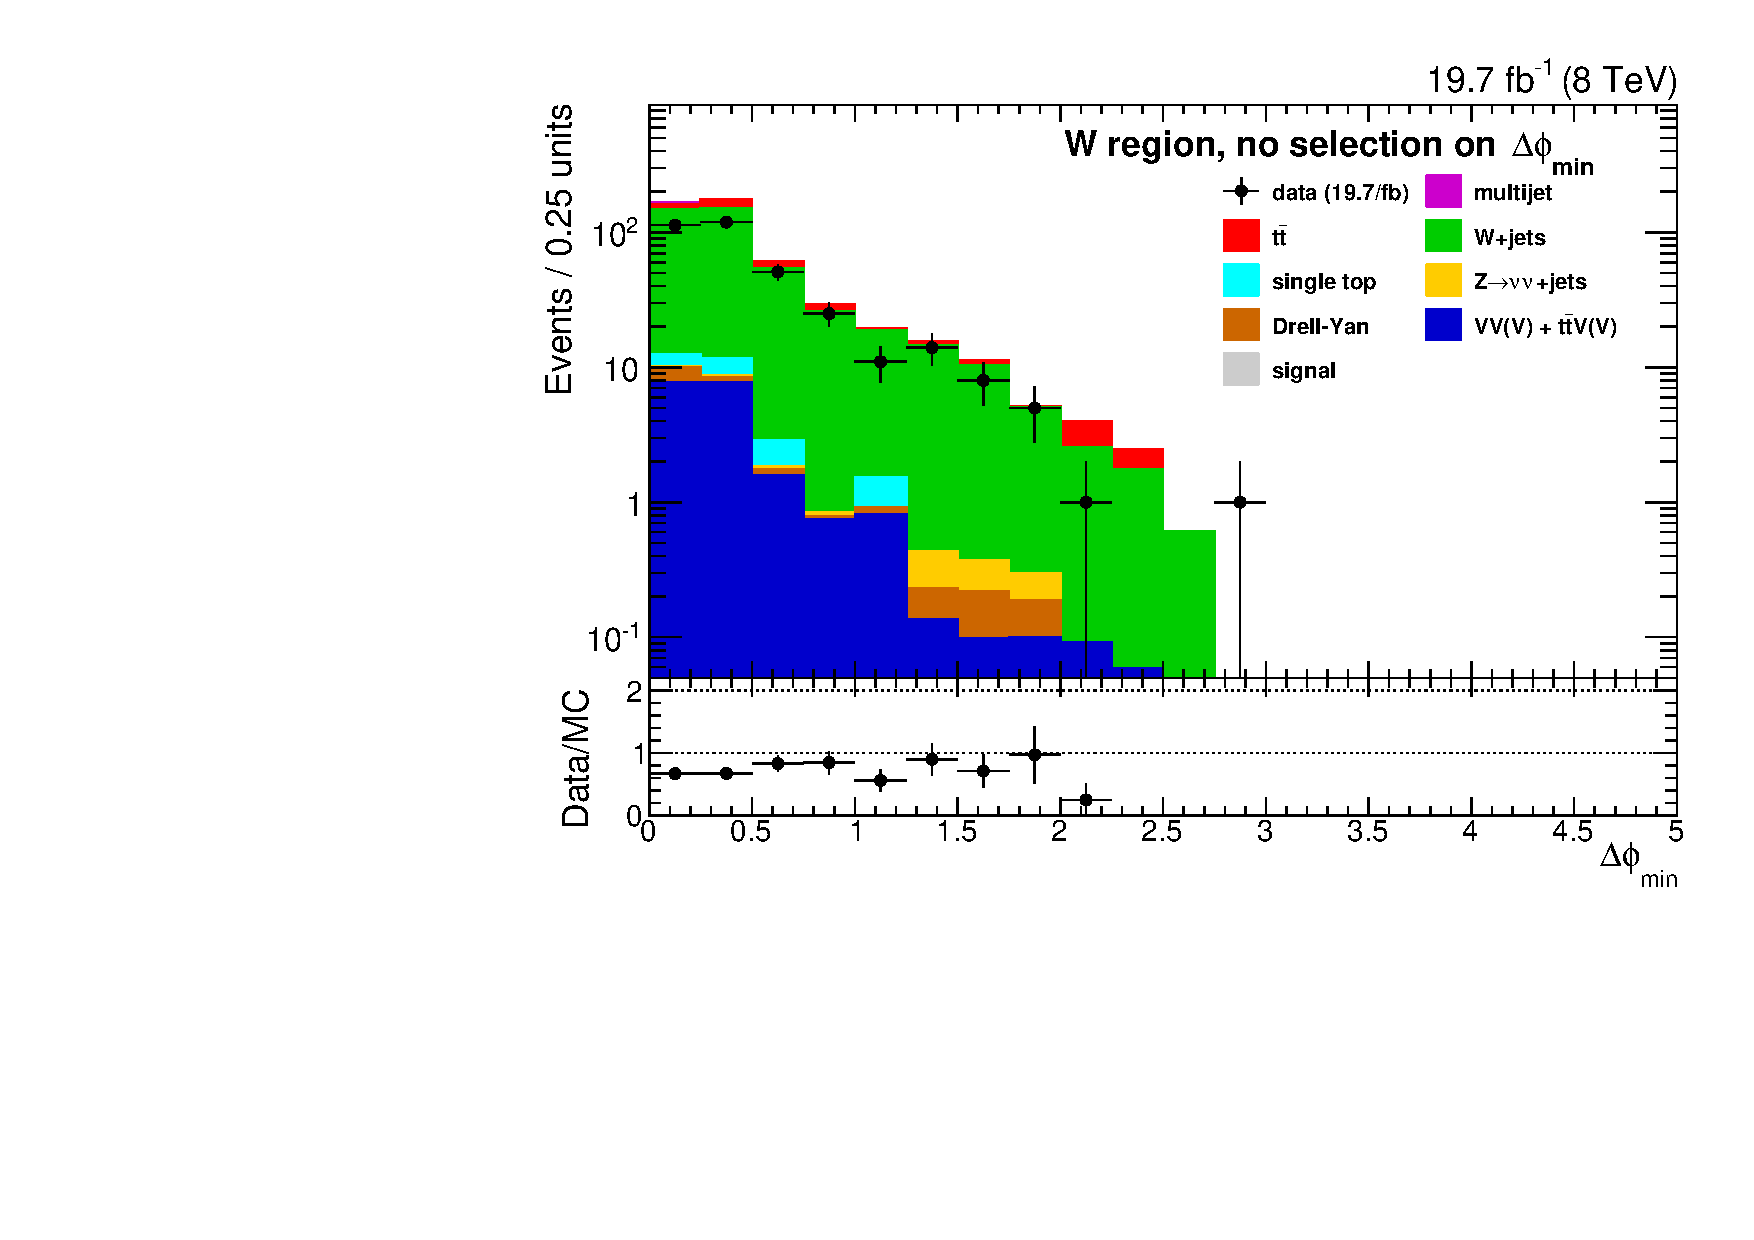
\includegraphics[width=0.6\textwidth]{figures/DataMC/DataMC_minDeltaPhi_0Lbg1Y1LlmT_rebin}
\caption{Comparison between data and simulation of the $\Delta\phi_{min}$ distribution in the $W$
region without any selection on $\Delta\phi_{min}$.
\label{fig:boost_W_region_mindeltaphi}}
\end{figure}

% In figure~\ref{fig:Shape_WJ_WvsS}, we show a comparison
% between the $M_R$ and $R^2$ shapes for Wjets simulation in the signal region versus the Wjets
% control region. The observed shapes are very similar. 
% 
\begin{figure}[htbp]
\centering
%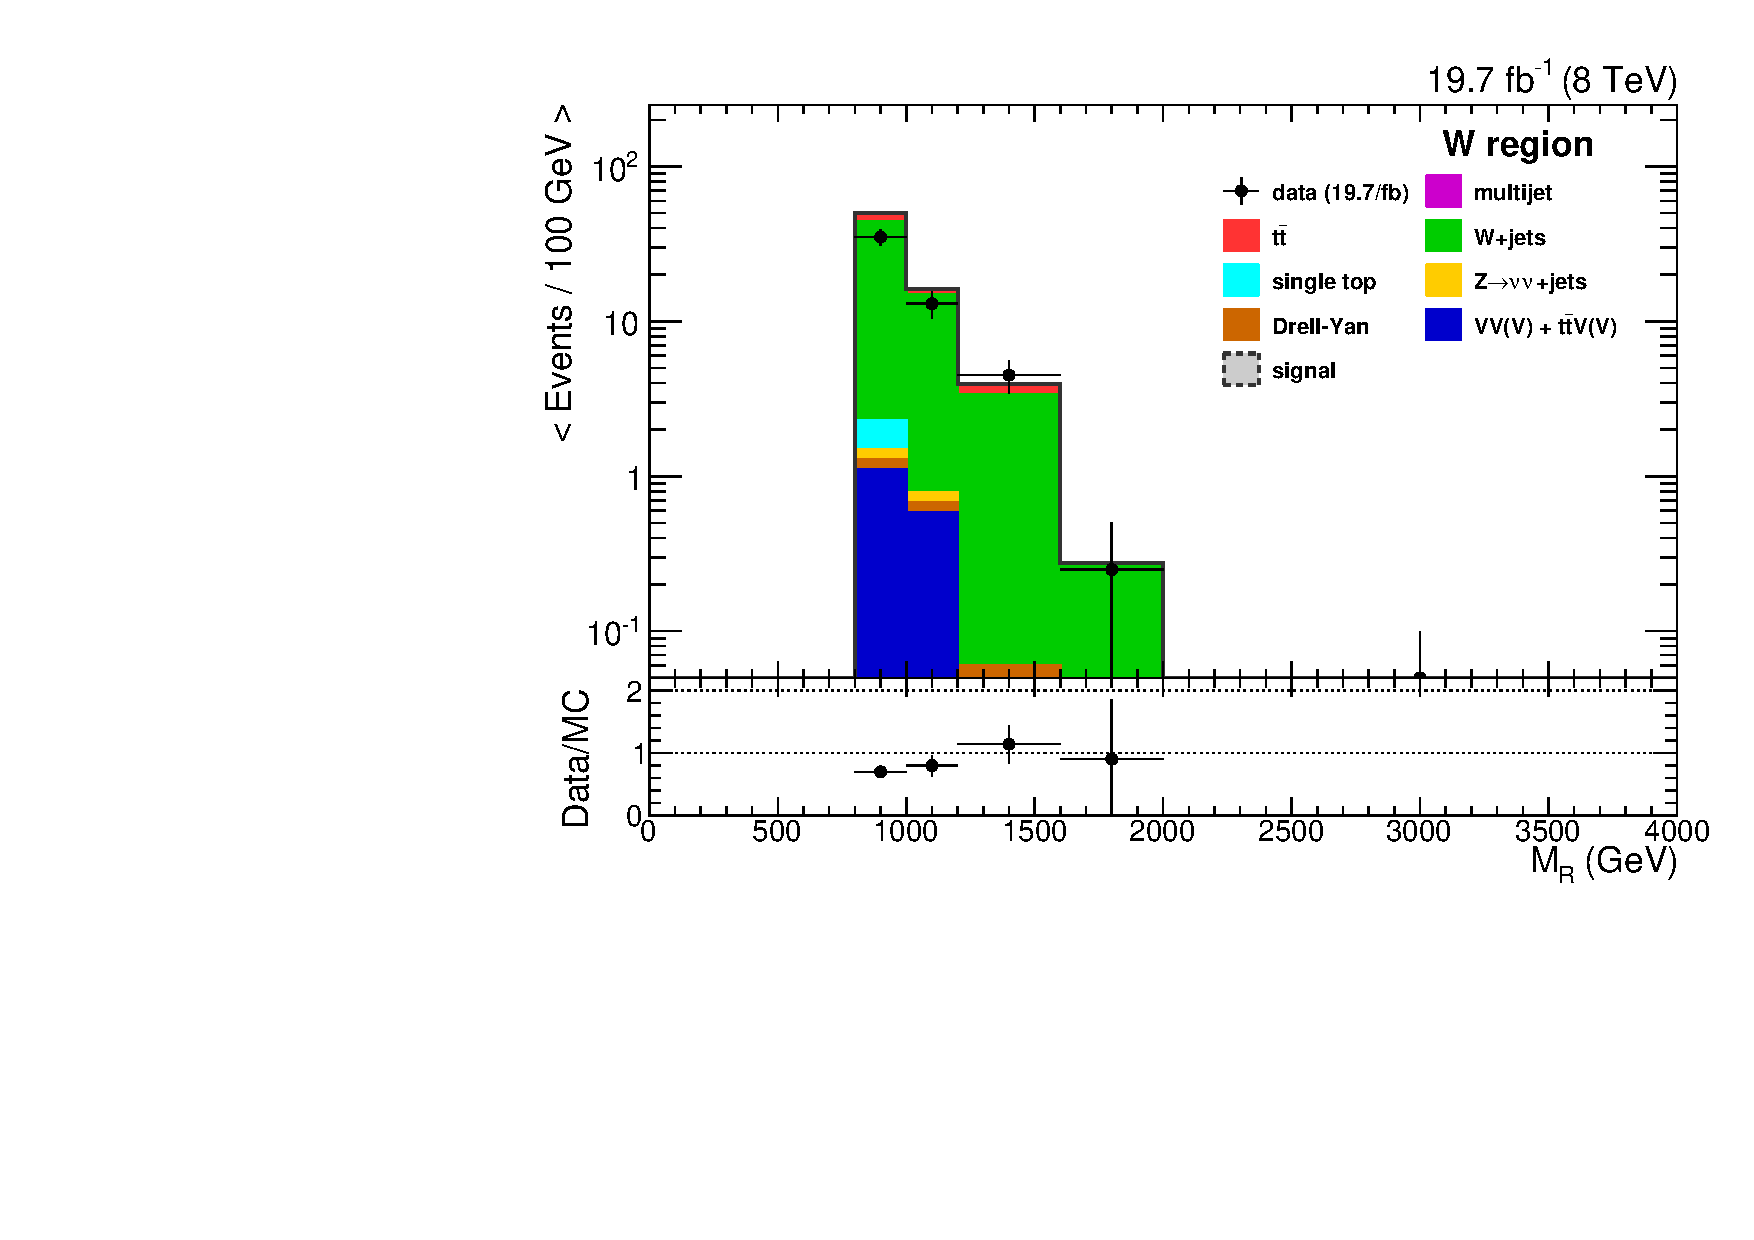
\includegraphics[width=0.48\textwidth]{figures/DataMC/DataMC_MR_0Lbg1Y1LlmT_mdPhig0p5_width}
%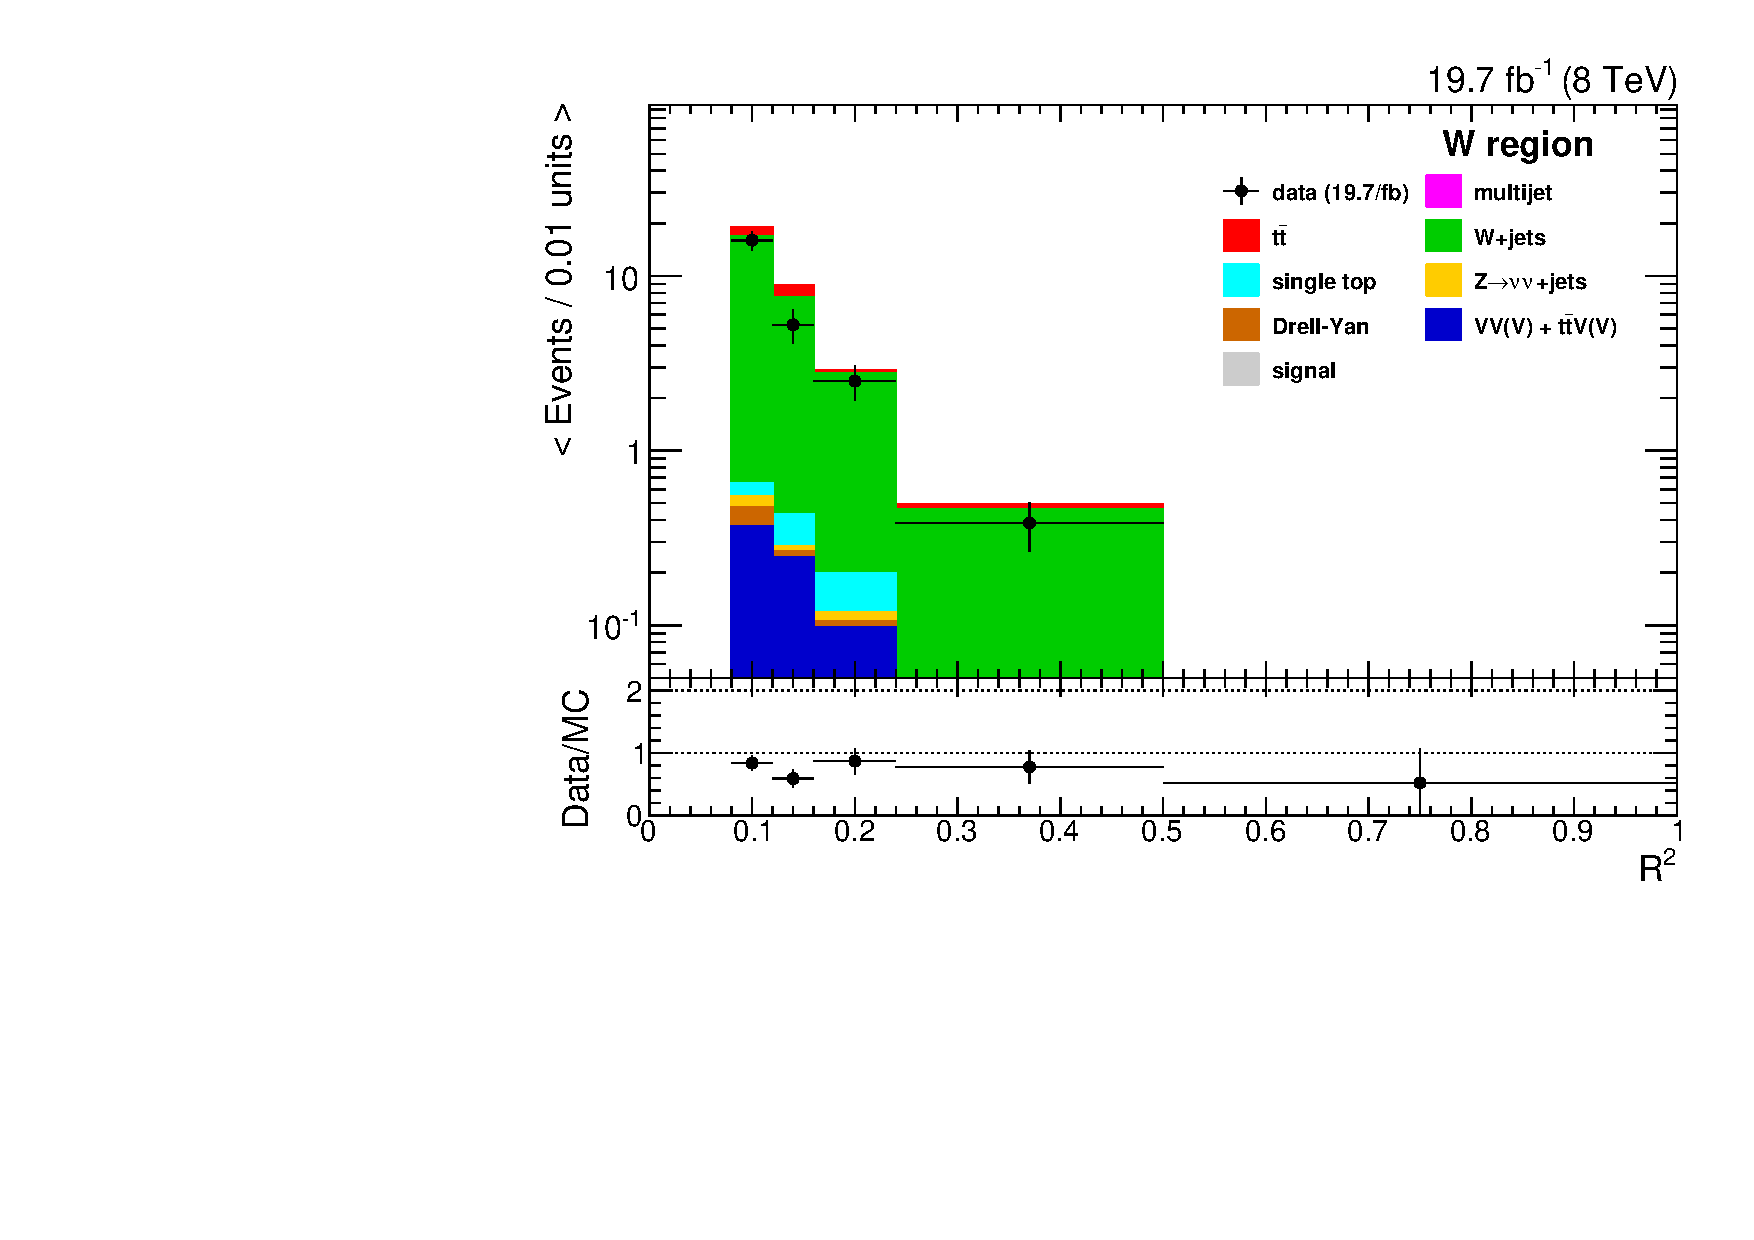
\includegraphics[width=0.48\textwidth]{figures/DataMC/DataMC_R2_0Lbg1Y1LlmT_mdPhig0p5_width}
\caption{Comparison between data and simulation of the $\mr$ (left) and $\rsq$ (right)
distributions in the $W$ region.
\label{fig:DataMC_WRegion_MR_R2_mdphig0p5}}
\end{figure}
% 
% 
% \begin{figure}[p]
% \centering
%  \includegraphics[width=0.49\textwidth]{figures/DataMC/DataMC_njets_0Lbg1Y1LlmT_mdPhig0p5}
% 
%  \includegraphics[width=0.49\textwidth]{figures/DataMC/DataMC_met_0Lbg1Y1LlmT_mdPhig0p5}
%  \includegraphics[width=0.49\textwidth]{figures/DataMC/DataMC_jet1pt_0Lbg1Y1LlmT_mdPhig0p5}
% 
%  \includegraphics[width=0.49\textwidth]{figures/DataMC/DataMC_jet2pt_0Lbg1Y1LlmT_mdPhig0p5}
%  \includegraphics[width=0.49\textwidth]{figures/DataMC/DataMC_jet3pt_0Lbg1Y1LlmT_mdPhig0p5}
% \caption{Data/MC comparison plot of various event quantities in the W region: 
% [top] jet multiplicity;
% [middle] missing transverse energy (left) and \pt of the highest \pt jet (right);
% [bottom] \pt of the second (left) and third (right) highest \pt jet. 
% \label{fig:DataMC_WRegion_mdphig0p5}}
% \end{figure}
% 
% \begin{figure}[htbp]
% \includegraphics[width=0.49\textwidth]{figures/Shapes/MR_comparison_WJ_WvsS_mdphi}
% \includegraphics[width=0.49\textwidth]{figures/Shapes/R2_comparison_WJ_WvsS_mdphi}
% \caption{Shape of $M_R$ (left) and $R^2$ (right) for $W+$jets simulation in the W region vs the S
% region. 
% \label{fig:Shape_WJ_WvsS}}
% \end{figure}

%%%%%%%%%%%%%%%%%%%%%%%%%%%%%%%%%%%%%%%%%%%%%%%%%%%%%%%%%%%%%%%%%%%%%%%%%%%%%%%%%%%%%%%%%%%%%%%%

\subsubsection{\texorpdfstring{$Q$}{Q} region}

The final background for which we define a control region, is QCD multijet production.
To define a region $Q$ enriched in multijet production, we start from the baseline selection, and
add the requirement that there be no loose lepton or isolated track present, as is the case for the
signal region selection. We also veto any event that contains a CSV loose $\cPqb$ tagged jet. 

Multijet events do not produce $\W$ bosons; any CA8 jet that passes the $\W$ boson tagger,
is thus by definition a misidentified $\W$ boson jet. To reach a similar kinematic phase space as
the signal region, we require that there be at least one $\W$ boson anti-tagged jet. The $\W$ boson
anti-tagging still requires that the jet mass is consistent with the $\W$ boson mass, but inverts
the N-subjettiness requirement. As we do not expect QCD multijet events to have the two-prong
jet-substructure of actual boosted $\W$ bosons, this will enhance the statistical power and purity
of the $Q$ region. 

As explained before, QCD multijet events are expected to have small values for the
$\Delta\phi_{min}$ variable. This can be seen from Fig.~\ref{fig:boost_Q_region_mindeltaphi}. 
For the $Q$ region definition we will thus reverse
and tighten the $\Delta\phi_{min}$ requirement from the signal region. We require $\Delta\phi_{min}
< 0.3$, which results in a very good purity of better than 90\% according to simulation. 
The full breakdown of the backgrounds according to simulation can again be found in
Tables~\ref{tab:cutflow} and \ref{tab:BG_comp_percent}.
Figure~\ref{fig:boost_Q_region_MR_Rsq} shows a comparison between data and simulation for the $\mr$
and $\rsq$ distributions. 
In figure~\ref{fig:boost_Q_region_shape}, we show a comparison between the shapes of the $\mr$ and
$\rsq$ distributions for the QCD multijet simulation in the signal region versus the $Q$ region. As
the statistical precision is quite limited for the multijet simulation in the signal region,
we also show in figure~\ref{fig:boost_Q_region_shape_no_mindeltaphi} the comparison for the $Q$ and
$S$ regions without selecting a particular $\Delta\phi_{min}$ region. The shape difference in this
region is smaller than when the $\Delta\phi_{min}$ cut is applied. We will assign a 40\% systematic
uncertainty on the multijet transfer factors in the background prediction to account for the
possible shape difference induced by the $\Delta\phi_{min}$ cut. 

% In reality this percentage will be even higher, as simulation is seen to underpredict the data in
% this control region. This is a known feature of the QCD multijet simulation, and its normalisation
% to LO cross sections. 


\begin{figure}[htbp]
\centering
%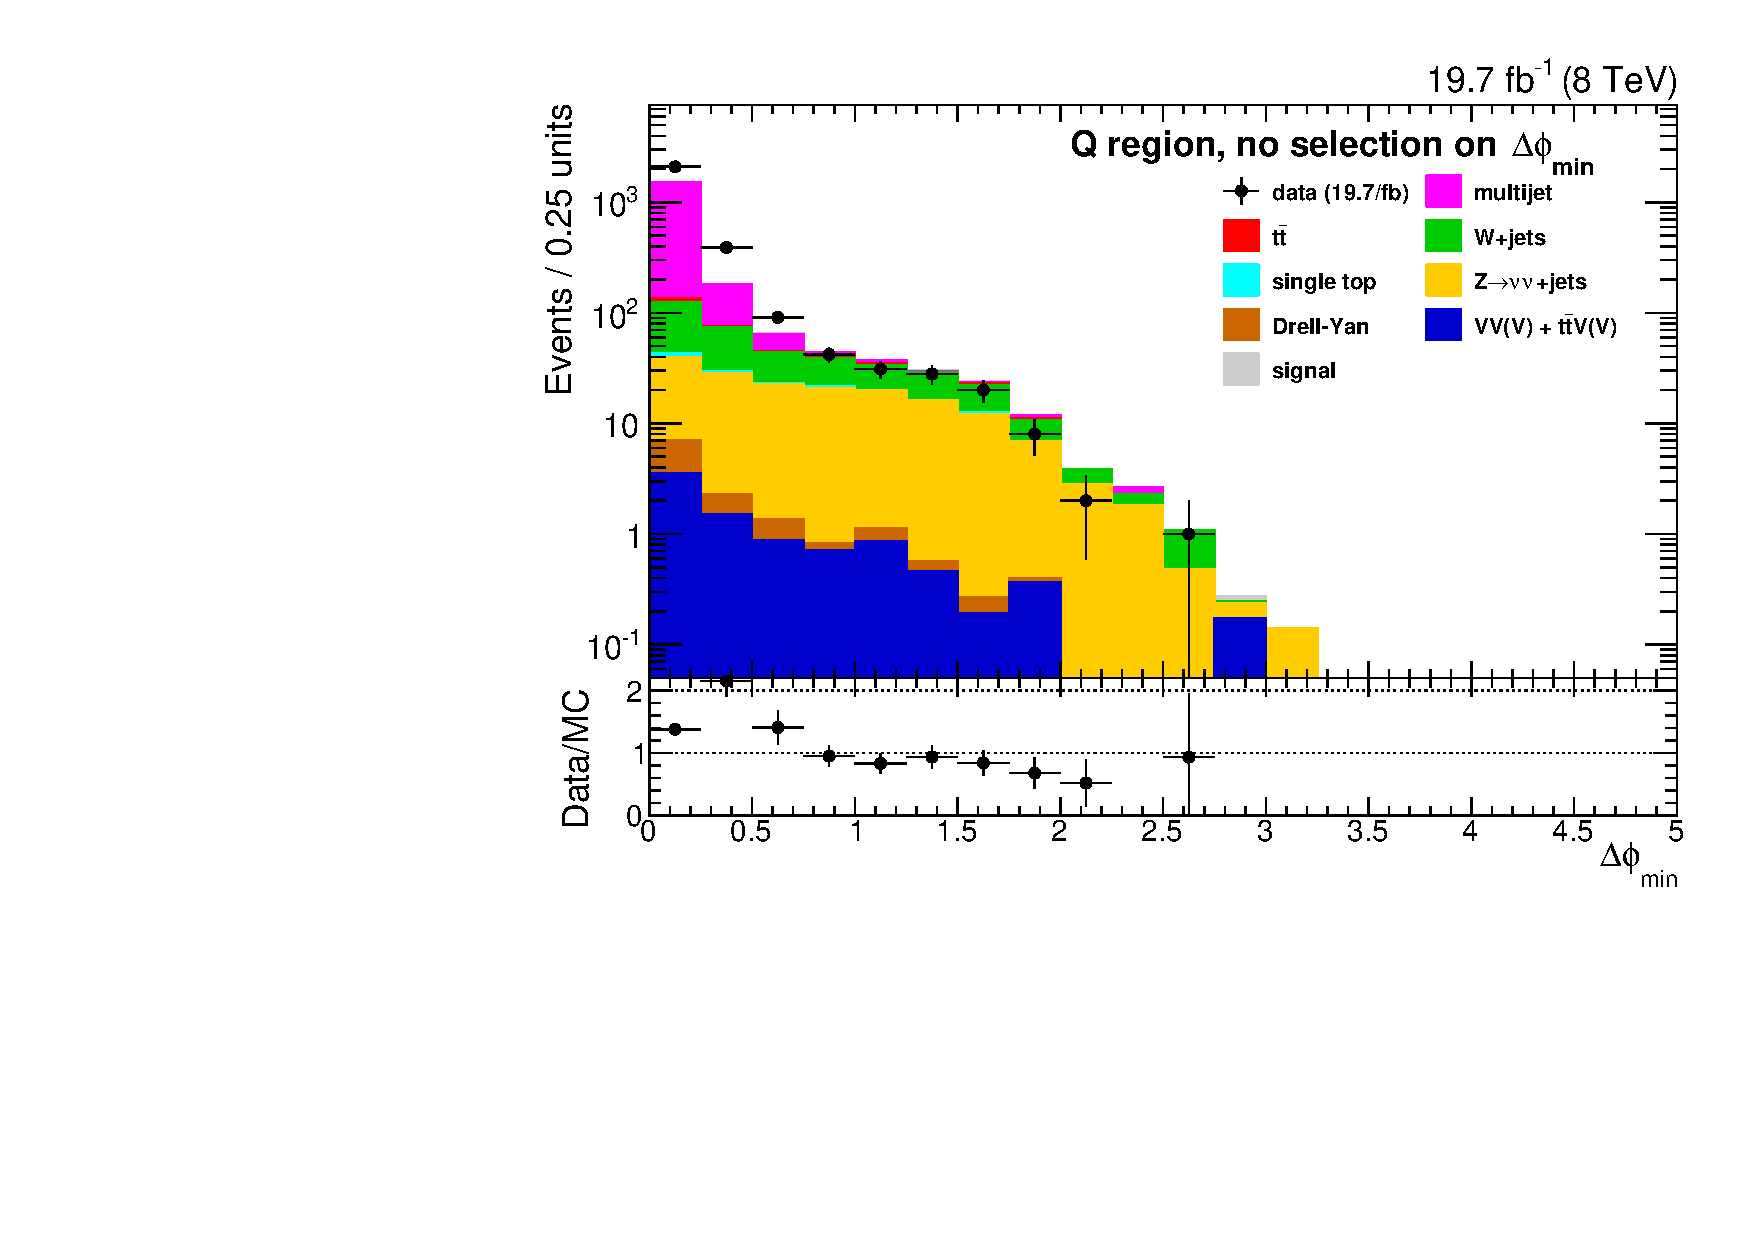
\includegraphics[width=0.6\textwidth]{figures/DataMC/DataMC_minDeltaPhi_0Lbg1uW0Ll_rebin}
\caption{Comparison between data and simluation of the $\Delta\phi_{min}$ distribution in the $Q$
region before any selection on $\Delta\phi_{min}$.
\label{fig:boost_Q_region_mindeltaphi}}
\end{figure}
% 
% Comparisons between data and simulation in the $Q$ region for $M_R$ and $R^2$ are shown in
% figure~\ref{fig:DataMC_QRegion_MR_R2_mdphi0p3}, and for various other basic quantities in
% figure~\ref{fig:DataMC_QRegion_mdphi0p3}. In figure~\ref{fig:Shape_QCD_QvsS}, we show a comparison
% between the $M_R$ and $R^2$ shapes for QCD simulation in the signal region versus the QCD control
% region. As the statistical precision is quite limited for the QCD simulation in the signal region,
% we also show in figure~\ref{fig:Shape_QCD_QvsS_nomdphi} the comparison for the $Q$ and $S$ regions
% without selecting a particular $\Delta\phi_{min}$ region. The shape difference in this region is
% smaller than when the $\Delta\phi_{min}$ cut is applied. We will assign a 40\% systematic
% uncertainty on the QCD related quantities in the background prediction to account for the possible
% shape difference induced by the $\Delta\phi_{min}$ cut. 
% 
\begin{figure}[htbp]
\centering
%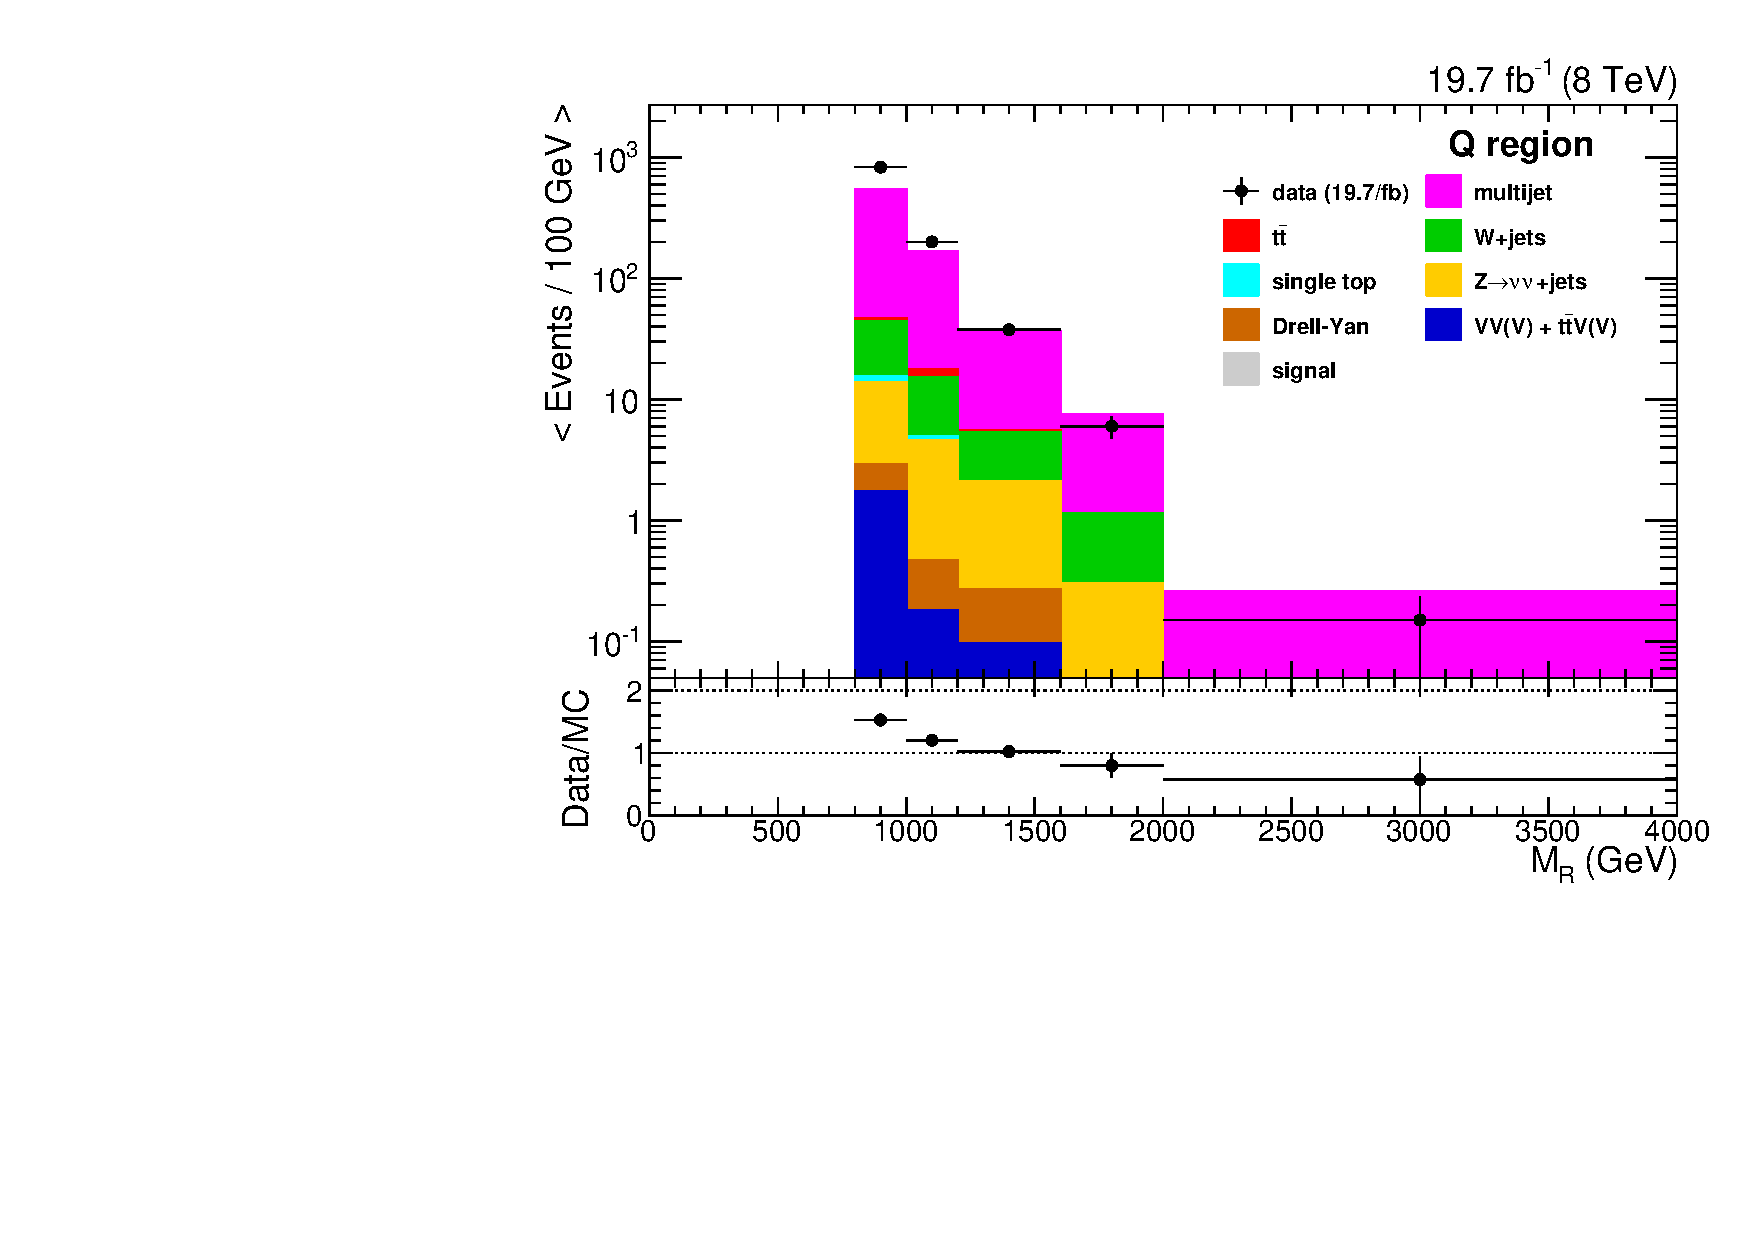
\includegraphics[width=0.48\textwidth]{figures/DataMC/DataMC_MR_0Lbg1uW0Ll_mdPhi0p3_width}
%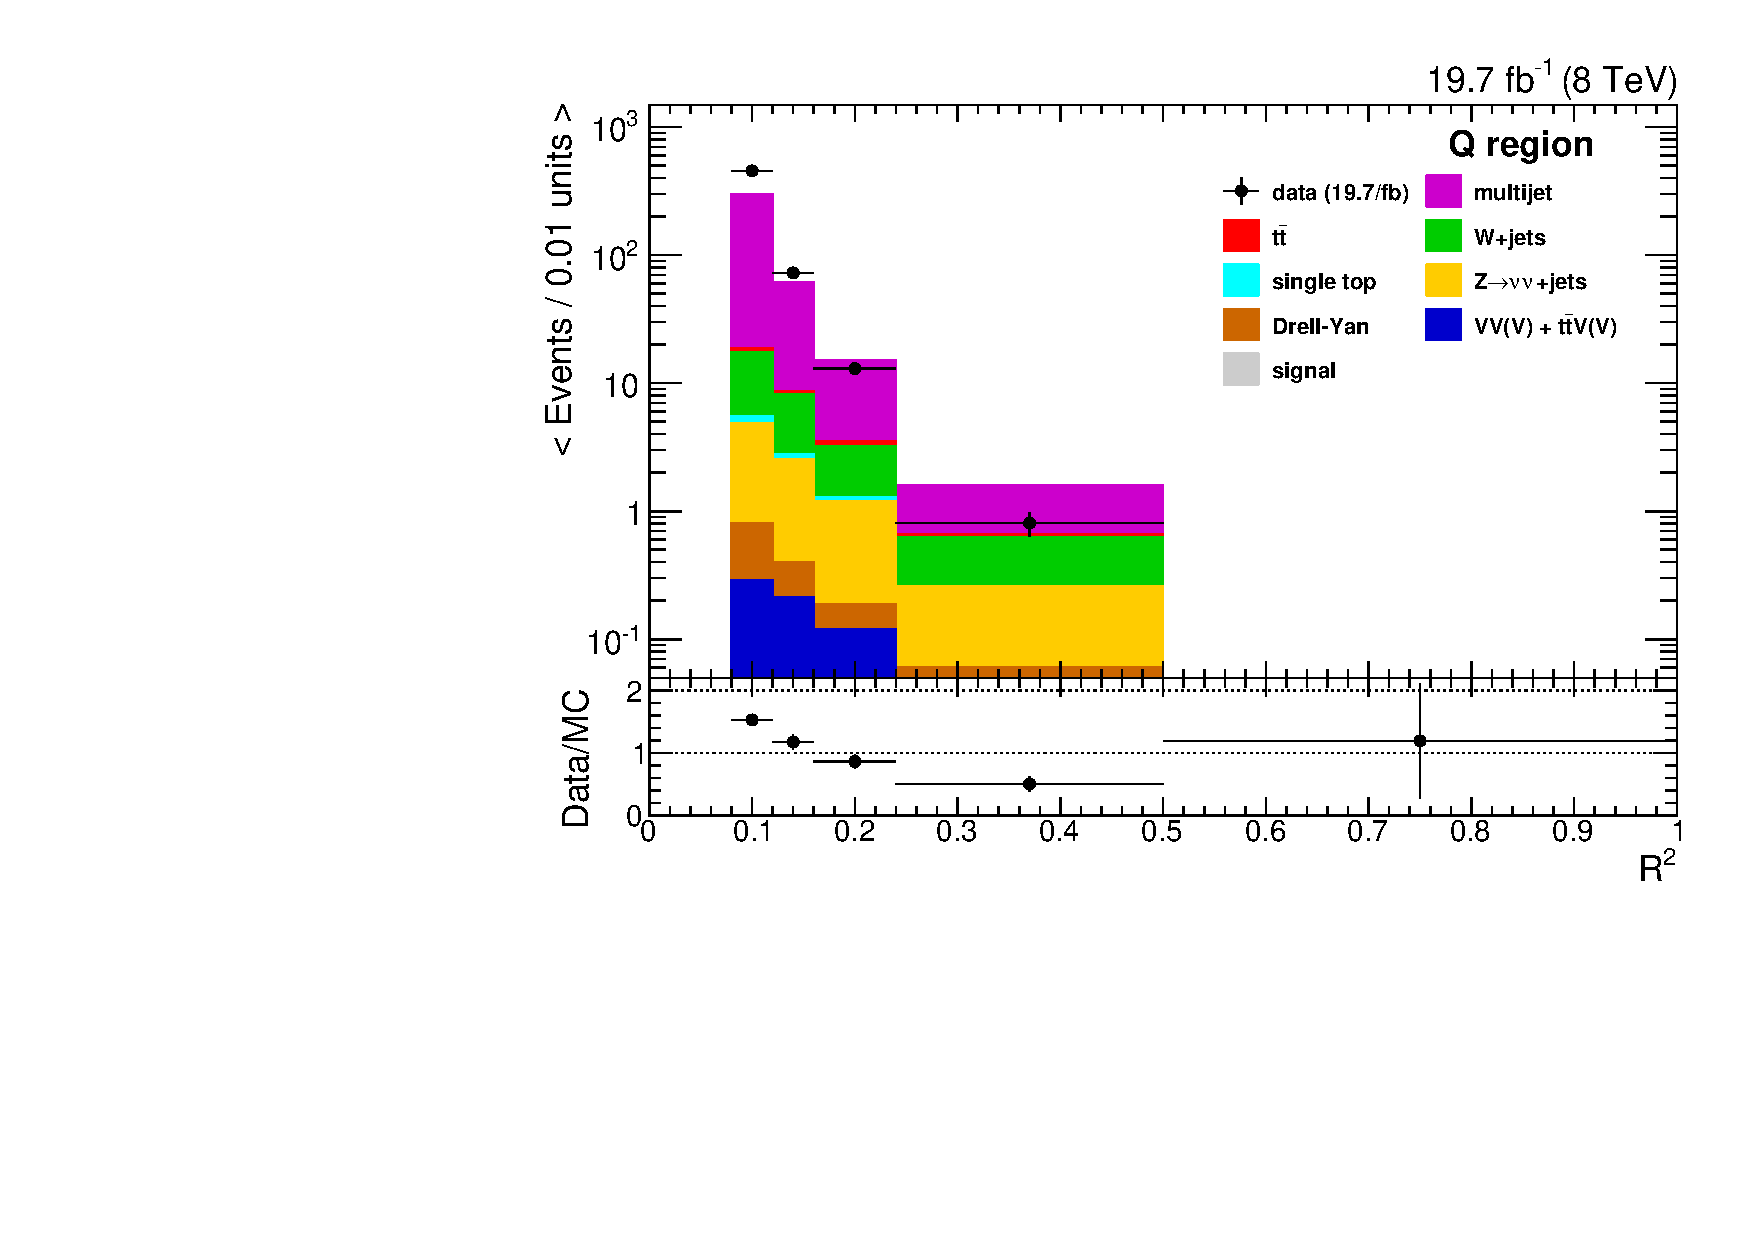
\includegraphics[width=0.48\textwidth]{figures/DataMC/DataMC_R2_0Lbg1uW0Ll_mdPhi0p3_width}
\caption{Comparison between data and simulation of the $\mr$ (left) and $\rsq$ (right)
distributions in the $Q$ region.
\label{fig:boost_Q_region_MR_Rsq}}
\end{figure}

% 
% \begin{figure}[p]
% \centering
%  \includegraphics[width=0.49\textwidth]{figures/DataMC/DataMC_njets_0Lbg1uW0Ll_mdPhi0p3}
% 
%  \includegraphics[width=0.49\textwidth]{figures/DataMC/DataMC_met_0Lbg1uW0Ll_mdPhi0p3}
%  \includegraphics[width=0.49\textwidth]{figures/DataMC/DataMC_jet1pt_0Lbg1uW0Ll_mdPhi0p3}
% 
%  \includegraphics[width=0.49\textwidth]{figures/DataMC/DataMC_jet2pt_0Lbg1uW0Ll_mdPhi0p3}
%  \includegraphics[width=0.49\textwidth]{figures/DataMC/DataMC_jet3pt_0Lbg1uW0Ll_mdPhi0p3}
% \caption{Data/MC comparison plot of various event quantities in the Q region: 
% [top] jet multiplicity;
% [middle] missing transverse energy (left) and \pt of the highest \pt jet (right);
% [bottom] \pt of the second (left) and third (right) highest \pt jet. 
% \label{fig:DataMC_QRegion_mdphi0p3}}
% \end{figure}

\begin{figure}[htbp]
\centering
%\includegraphics[width=0.48\textwidth]{figures/Shapes/MR_comparison_QCD_QvsS_mdphi}
%\includegraphics[width=0.48\textwidth]{figures/Shapes/R2_comparison_QCD_QvsS_mdphi}
\caption{Shape of the $\mr$ (left) and $\rsq$ (right) distribution for the QCD multijet simulation
in the $Q$ region versus the $S$ region. 
\label{fig:boost_Q_region_shape}}
\end{figure}

\begin{figure}[htbp]
\centering
%\includegraphics[width=0.48\textwidth]{figures/Shapes/MR_comparison_QCD_QvsS_no_mdphi}
%\includegraphics[width=0.48\textwidth]{figures/Shapes/R2_comparison_QCD_QvsS_no_mdphi}
\caption{Shape of the $\mr$ (left) and $\rsq$ (right) distribution for the QCD multijet simulation
in the $Q$ region versus the $S$ region with the requirement on  $\Delta\phi_{min}$ removed in both
regions. 
\label{fig:Shape_QCD_QvsS_nomdphi}}
\end{figure}



\begin{table}[thbp]
\centering
\caption{Summary of selection for signal and control regions.
These requirements are in addition to the baseline selection. \label{tab:boost_selection_summary}}
\vspace{1ex}
\begin{tabular}{lccccc}
\toprule
Selection & $S$ region & $S'$ region & $Q$ region & $T$ region & $W$ region \\ 
\midrule
nr of $\cPqb$ jets        & ${\geq}\, 1$   & ${\geq}\, 1$   & 0        & ${\geq}\, 1$      & 0
\\
nr of mass-tagged $\W$'s & ${\geq}\, 1$   & ${\geq}\, 1$   & ${\geq}\, 1$ & ${\geq}\, 1$     
&
${\geq}\, 1$ \\
nr of tagged $\W$'s      & ${\geq}\, 1$   & ${\geq}\, 1$   & -        & ${\geq}\, 1$      & -
\\
nr of anti-tagged $\W$'s & -          & -          & ${\geq}\, 1$ & -             & - \\
nr of loose leptons       & 0          & 0          & 0        & 1             & 1 \\
nr of isolated tracks        & 0          & 0          & 0        & -             & - \\
$m_T$                         & -          & -          & -        & ${<}\,100$\GeV   &
30--100\GeV\\
$\Delta\phi_{min}$            & ${>}\, 0.5$    & ${<}\, 0.5$    & ${<}\, 0.3$  & ${>}\, 0.5$      
&
${>}\, 0.5$\\
\bottomrule
\end{tabular}
\end{table}

\begin{sidewaystable}[p]
\centering
\caption{Cutflow table, event counts are normalized to $19.7\fbinv$. The signal is the
$m_{\tilde{g}}=1000\GeV$, $m_{\stopone}=325\GeV$, $m_{\lsp}=300\GeV$ point of the
T1ttcc scan. The row corresponding to ``$n_{PV} > 0$'' gives the event counts after applying the
cleaning filters, pileup reweighting, top \pt reweighting for $t\bar{t}$, ISR reweighting for
signal, and the requirement of at least one good primary vertex. The column indicating the total
number of events also includes some smaller processes that only contribute at the early stages of
the event selection. 
The cross sections used for each sample are listed in the second row.}
\vspace{1ex}
{\scriptsize
\begin{tabular}{ l | c  c  c  c  c  c  c  c  c | c  c  c }
%\begin{tabular}{ l || c  c  c  c  c  c  c  c  c | c || c || c }
%\begin{tabular}{| l || c | c | c | c | c | c | c | c | c | c || c || c || c |}
\toprule
Selection & Multijet & $t\bar{t}$ & $\W{\rightarrow}\ell\nu+$jets & Diboson & Single top &
$\cPZ{\rightarrow}\nu\nu+$jets & DY${\rightarrow}\ell\ell+$jets & Triboson & $t\bar{t}V$ & Total &
Signal & Data\\ 
 & $10.4\times 10^7$ pb & 245.8 pb & 111.5 pb & 95.4 pb & 114.9 pb & 588.3 pb & 22.6 pb & 0.69 pb &
1.88 pb & & 0.02435 pb & \\ 
 \midrule
% & 10.4e+07 pb & 245.8 pb & 111.5 pb & 95.4 pb & 114.9 pb & 588.3 pb & 22.6 pb & 0.69 pb & 1.88 pb & 121 pb & & 0.0243547 pb & \\ \hline \hline
No selection & $2.1\times 10^{11}$ & $4.9\times 10^6$ & $2.2\times 10^6$ & $1.9\times 10^6$ & $2.3\times 10^6$ & $1.2\times 10^7$ & $4.5\times 10^5$ & $1.2\times 10^4$ & $3\times 10^4$ & $2.1\times 10^{11}$ & 499 &  \\
$n_{PV} > 0$ & $1.05\times 10^{11}$ & $4.42\times 10^6$ & $2.02\times 10^6$ & $1.08\times 10^6$ & $1.72\times 10^6$ & $2.87\times 10^6$ & $3.7\times 10^5$ & $8.46\times 10^3$ & $2.6\times 10^4$ & $1.05\times 10^{11}$ & 479 & \\
$n_j \geq 3$ & $2.04\times 10^{10}$ & $4.08\times 10^6$ & $1.51\times 10^6$ & $5.19\times 10^5$ & $1.10\times 10^6$ & $6.24\times 10^5$ & $3.06\times 10^5$ & $5.64\times 10^3$ & $2.49\times 10^4$ & $2.05\times 10^{10}$ & 472 &  \\
$\pt(j_1) > 200\GeV$ & $1.82\times 10^8$ & $2.88\times 10^5$ & $4.36\times 10^5$ & $1.86\times 10^4$ & $6.08\times 10^4$ & $5.89\times 10^4$ & $6.61\times 10^4$ & 924 & $5.24\times 10^3$  & $1.82\times 10^8$ & 403 & \\
$M_R \,{>}\, 800, R^2 \,{>}\, 0.08$ & $3.47\times 10^4$ & $5.83\times 10^3$ & $1.17\times 10^4$ & 309 & 900 & $3.25\times 10^3$ & 422 & 40.2 & 183 & 57557 & 224 & \\
Trigger & $3.15\times 10^4$ & $5.12\times 10^3$ & $9.38\times 10^3$ & 249 & 786 & $2.32\times 10^3$ & 367 & 36.4 & 166 & 50164 & 216 & 67037 \\
\midrule
no lepton & $3.09\times 10^4$ & $1.87\times 10^3$ & $3.75\times 10^3$ & 96.3 & 311 & $2.30\times 10^3$ & 145 & 12.6 & 58.5 & 39666 & 142 & 56220 \\
\midrule[.02em]
$n_b \geq 1$ & $9.37\times 10^3$ & $1.51\times 10^3$ & 590 & 25.2 & 226 & 302 & 29.0 & 4.48 & 46.3 & 12187 & 119 & 18164 \\
$n_W \geq 1$ & 841 & 332 & 56.4 & 8.52 & 56.7 & 22.1 & 5.28 & 1.98 & 9.68 & 1350 & 28 & 1817  \\
S & 14.8 & 90.4 & 23.1 & 3.7 & 11.7 & 12.7 & 0.59 & 0.98 & 2.6 & 160 & 23.4 & 187 \\
\midrule[.02em]
$n_b = 0$ & $1.25\times 10^4$ & 98.3 & $1.70\times 10^3$ & 35.6 & 25.9 & $1.25\times 10^3$ & 46.5 & 4.19 & 3.56 & 15691 & 5.65 & 20667 \\
$n_{aW} \geq 1$ & 1519 & 18.7 & 204 & 8.36 & 7.40 & 158 & 5.41 & 0.751 & 0.819 & 1923 & 0.667 & 2712 \\
Q & 1447 & 10.6 & 93.1 & 3.88 & 3.94 & 38.9 & 3.68 & 0.28 & 0.52 & 1603 & 0.07 & 2240 \\
\midrule
1 lepton & 585.9 & $2.74\times 10^3$ & $5.52\times 10^3$ & 132 & 421 & 22.1 & 164 & 19.2 & 88.5 & 9699 & 65.0 & 10008 \\
\midrule[.02em]
$n_b \geq 1$ & 236.7 & $2.17\times 10^3$ & 625 & 29.9 & 301 & 4.14 & 28.7 & 5.36 & 68.3 & 3470 & 54 & 3930 \\
$n_W \geq 1$ & 24.3 & 496 & 61.6 & 10.0 & 50.9 & 0.56 & 3.57 & 2.36 & 16.0 & 666 & 12.3 & 770 \\
T & 0 & 112 & 20.2 & 2.0 & 13.3 & 0 & 0.38 & 0.50 & 3.2 & 151 & 1.2 & 153 \\
\midrule[.02em]
$n_b = 0$ & 150.5 & 153 & $2.86\times 10^3$ & 52.8 & 41.3 & 11.5 & 55.8 & 7.05 & 5.94 & 3329 & 2.54 & 3165 \\
$n_Y \geq 1$ & 30.8 & 79.1 & 605 & 33.1 & 13.8 & 2.4 & 13.1 & 4.57 & 2.61 & 786 & 1.19 & 581 \\
W & 0 & 15.5 & 127 & 3.6 & 1.6 & 0.64 & 0.59 & 0.52 & 0.29 & 150 & 0.06 & 116 \\
\bottomrule
\end{tabular}
}
\label{tab:cutflow}
\end{sidewaystable}

\begin{table}[htpb]
\centering
\caption{Background composition according to simulation
\label{tab:BG_comp_percent}}
\vspace{1ex}
{\small
\begin{tabular}{ l  c  c  c  c  c  c  c }
\toprule
Selection & Multijet & $t\bar{t}$ & $\W(\rightarrow \ell\nu)+$jets & Single top & $\cPZ(\rightarrow
\nu\bar{\nu})+$jets & Diboson & Other \\  
\midrule
Baseline & 62.8\% & 10.2\% & 18.7\% & 1.6\% & 4.6\% & 0.5\% & 1.6\% \\ 
$S$ & 9.2\% & 56.3\% & 14.4\%  & 7.3\% & 7.9\% & 2.3\% & 2.6\% \\
$Q$ & 90.2\% & 0.7\% & 5.8\%  & 0.2\% & 2.4\% & 0.2\% & 0.3\% \\
$T$ & 0.0\% & 73.9\% & 13.3\%  & 8.8\% & 0.0\% & 1.3\% & 2.7\% \\
$W$ & 0.0\% & 10.3\% & 84.8\%  & 1.1\% & 0.4\% & 2.4\% & 1.0\% \\
\bottomrule
\end{tabular}
}
\end{table}


